\subsection{Dalvik Executionable File Format} \label{subsection:android-dex}
As explained in subsection~\ref{subsection:foundation-android-package}, Android applications are distributed using \gls{apk}s.
They contain the application code as Dalvik bytecode that has been compiled from the Java source code.
\newline
Dalvik bytecode is suited to run on the ARM architecture.
It supports direct mapping from dex registers to the 32 bit registers of the ARM processor.
The opcodes are 16 bit, which makes the dex bytecode less compact than Java bytecode with its 8 bit instructions.
The 16 bit opcodes result in 218 valid opcodes which have a source-dest ordering for its arguments.
Instructions are 16 bit multiples and at least 32 bit large with opcode and argument combined.
An example is the hex presentation of instruction to move a 4 bit constant into a variable,  \textit{12 iv}.
It is 32 bit long and contains the 16 bit opcode \textit{12}, \textit{const/4}, the source 4 bit constant \textit{i} and the destination variable \textit{v}  \cite{opcodes}.
In case there are larger than 32 bit instructions, adjacent registers are used to store it. \cite{androidDalvik}
\newline
Similar to Java bytecode, values are not stored inside the method but as a reference pointing to the location.
While in Java each class has its constants, like numbers, strings and identifier names, grouped together in heterogenous pool (see figure figure~\ref{fig:java}, left side), Dalvik bytecode uses one pool for each type.
When compiling Java bytecode to Dalvik bytecode, the heterogenous pools of each Java class are merged into one global pool for each type (see figure figure~\ref{fig:java}, right side).
The merging of pool allows to remove duplicates and point their reference to only one value.
This reduces the memory need for constant but increases the number of references.
This approach is most effective for strings.
A decrease of the memory footprint of up to 44\% compared to the \gls{jar} is possible.
\newline
\begin{figure}[h]
    \centering
    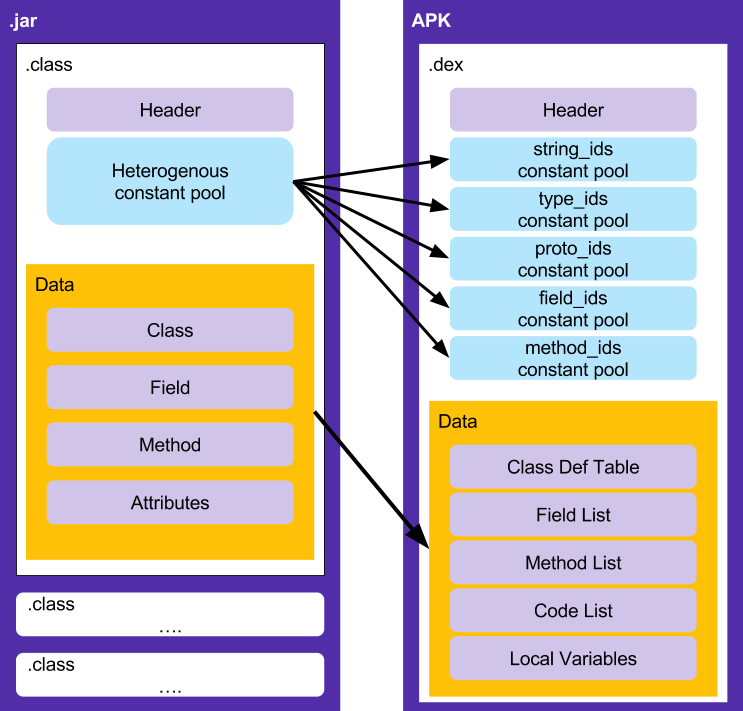
\includegraphics[width=0.5\textwidth]{data/java.png}
    \caption{\gls{jar} to \gls{apk} transformation \cite{googleDalvik}}
    \label{fig:java}
\end{figure}
The compiled \gls{dex} file has the the structure seen in figure~\ref{fig:dex} on the left.
Most important parts of the header are the checksum and the signature.
The checksum field contains the Adler32 checksum of the \gls{dex} file. It is calculated from everything all fields of the file except the magic field and itself.
The checksum is used to detect whether the file is corrupt.
The signature field contains the SHA-1 hash value of the file.
It is based on every field except the magic field, checksum field and itself.
The file can be uniquely identified by the signature.
It is part of the file signing and stored in the manifest files to ensure integrity and authenticity.
When the file is modified, both values have to be recalculated and updated.
\cite{developersDalvik} \cite{ehringerDalvik}
\newline
\begin{figure}[h]
    \centering
    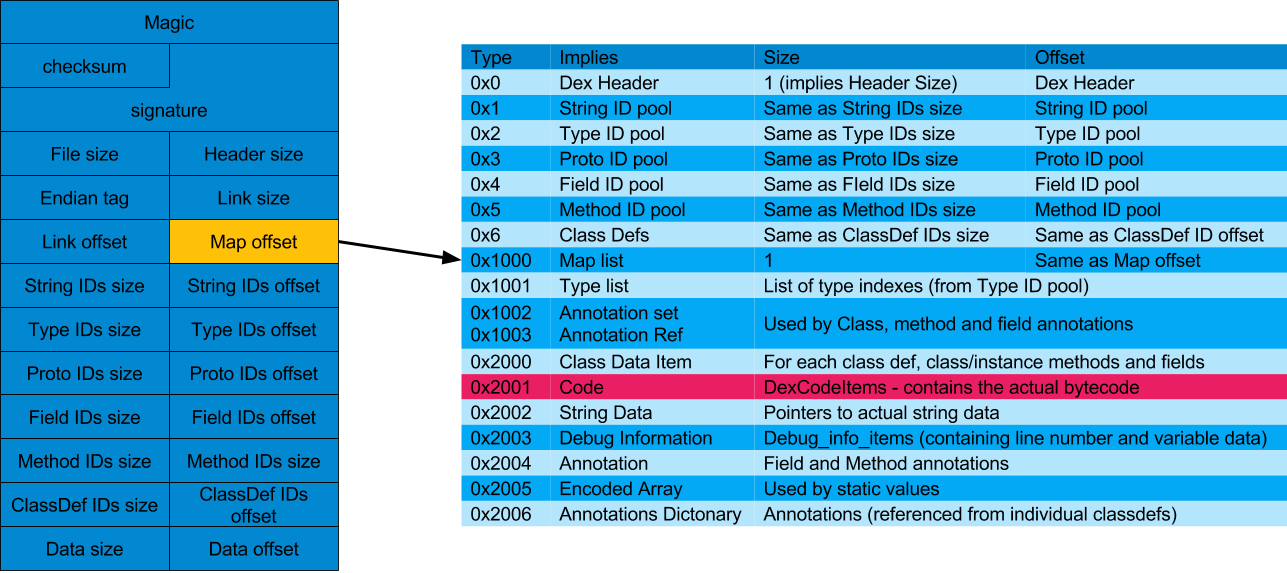
\includegraphics[width=0.8\textwidth]{data/dex.png}
    \caption{\gls{dex} file format \cite{andevconDalvikART}}
    \label{fig:dex}
\end{figure}
Dex bytecode supports optimization.
Upon installation improvements specific to the underlying architecture can be applied to the bytecode.
The resulting \gls{dex} file is called \gls{odex}.
The optimization is executed by a program called \textit{dexopt} which is part of the Android platform.
The semantics of the two files is the same, but the \gls{odex} file has the better performance.
\newline
Like Java bytecode, \gls{dex} bytecode has a serious flaw.
Since bytecode is pretty simple and contains a lot of meta information, decompilation can be done and the result is easily understandable.
At the same time, protection is rarely applied by the developers.
This makes these applications an easy target for reverse engineering.
